\graphicspath{{chapter6/figures/}}
\chapter{Seg-metrics: a Python package to compute segmentation metrics}
\label{chap:6}

% This is for title at the border of the page
\runningchaptertitle{seg-metrics}

% This is an example to put the publication
\publishedat{}{\textbf{Jia, J.} \textbf{A package to compute segmentation metrics: seg-metrics}. onlline at \textit{https://pypi. org/project/seg-metrics} (2020).} 

\ThumbIndexShow
%---------------------------------------

\begin{abstract}

\end{abstract}

\clearpage

\section{Background}

\section{Related packages}
As far as we know, there are two open source packages for segmentation metrics calculation. The first package is 

\section{Our \texttt{seg-metrics} package}

\subsection{Overlap based metrics}
    
\url{https://en.wikipedia.org/wiki/Confusion_matrix}

\begin{itemize}

\item Dice Coefficient (F1-Score)
\begin{equation}
Dice = \frac{2 \times |A \cap B|}{|A| + |B|} = \frac{2 \times TP}{2 \times TP + FP + FN}
\end{equation}



\item Jaccard index
\begin{equation}
Jaccard = \frac{|A \cap B|}{|A \cup B|} = \frac{TP}{TP + FP + FN}
\end{equation}

\item Precision/Positive predictive value (PPV)

Precision score is the number of true positive results divided by the number of all positive results
\begin{equation}
Precision = \frac{TP}{TP + FP}
\end{equation}

\item Selectivity/Specificity/True negative rate
\begin{equation}
Specificity = \frac{TN}{TN + FP}
\end{equation}


\item Recall/Sensitivity/Hit rate/True positive rate (TPR)

Recall score, also known as Sensitivity, hit rate, or TPR, is the number of true positive results divided by the number of all samples that should have been identified as positive

\begin{equation}
Sensitivity = \frac{TP}{TP + FN}
\end{equation}


\item Accuracy/Rand Index

Accuracy score, also known as Rand index is the number of correct predictions, consisting of correct positive and negative predictions divided by the total number of predictions.
\begin{equation}
    Accuracy = \frac{TP + TN}{TP + FP + FN + TN}
\end{equation}

\end{itemize}

\subsection{Distance based metrics}
Hausdorff distance (HD)
\begin{equation}
HD = \max \left\{ \sup_{a \in A} \inf_{b \in B} d(a, b), \sup_{b \in B} \inf_{a \in A} d(b, a) \right\}
\end{equation}
where $sup$ represents the supremum operator, $inf$ is the infimum operator, and $inf_{b \in B} d(a, b)$ quantifies the distance from a point $a \in X$ to the subset $B \subseteq X$.

Hausdorff distance 95\% percentile (HD95)

Mean (Average) surface distance (MSD)

Median surface distance (MDSD)


\section{Use cases}

\texttt{seg-metrics} is a Python package which output the segmentation metrics by receiving one ground truth image and another predicted image. After we import the package by \texttt{from seg\_metrics import seg\_metrics}, the syntax to use it is as follow (\textbf{Note:} all the following cases are based on texttt{seg-metrics 1.1.6}).
\begin{minted}
[frame=single]
{python}
write_metrics(labels,
              gdth_path = None,
              pred_path = None,
              csv_file = None,
              gdth_img = None,
              pred_img = None,
              metrics = None,
              verbose = False,
              spacing = None,
              fully_connected = True,
              TPTNFPFN = False)
    """ Parameter description.
    labels: a list of labels to performe the calculation of metrics.
    gdth_path: a (sequence of) path of ground truth.
    pred_path: a (sequence of) path of prediction.
    csv_file: filename to save the metrics.
    gdth_img: a (sequence of) ground truth.
    pred_img: a (sequence of) prediction.
    metrics: metric names.
    verbose: whether to show the animated progress bar
    spacing: spacing of input images.
    fully_connected: whether to apply fully connected border.
    TPTNFPFN: whether to return the confusion matrix.
    
    return: A dict or a list of dicts which store metrics.
    """
\end{minted}

More examples are shown below.

\begin{itemize}
    \item Evaluate two batches of images with same filenames from two different folders.

\begin{minted}
[frame=single]
{python}
labels = [4, 5 ,6 ,7 , 8]
gdth_path = 'data/gdth'  # folder for ground truth images
pred_path = 'data/pred'  # folder for predicted images
csv_file = 'metrics.csv'  # file to save results

metrics = sg.write_metrics(labels=labels,
                  gdth_path=gdth_path,
                  pred_path=pred_path,
                  csv_file=csv_file)
print(metrics)  
\end{minted}

        \item Evaluate two images

\begin{minted}
[frame=single]
{python}
labels = [4, 5 ,6 ,7 , 8]
gdth_file = 'data/gdth.mhd'  # full path for ground truth image 
pred_file = 'data/pred.mhd'  # full path for prediction image
csv_file = 'metrics.csv'

metrics = sg.write_metrics(labels=labels,
                           gdth_path=gdth_file,
                           pred_path=pred_file,
                           csv_file=csv_file)
\end{minted}

        \item Evaluate two images with specific metrics


\begin{minted}
[frame=single]
{python}
labels = [0, 4, 5 ,6 ,7 , 8]
gdth_file = 'data/gdth.mhd'
pred_file = 'data/pred.mhd'
csv_file = 'metrics.csv'

metrics = sg.write_metrics(labels=labels[1:],
                  gdth_path=gdth_file,
                  pred_path=pred_file,
                  csv_file=csv_file,
                  metrics=['dice', 'hd'])
# for only one metric
metrics = sg.write_metrics(labels=labels[1:], 
                  gdth_path=gdth_file,
                  pred_path=pred_file,
                  csv_file=csv_file,
                  metrics='msd')  
\end{minted}

\item Select specific metrics.
By passing the following parameters to select specific metrics.

\begin{minted}
[frame=single]
{python}
# ----------Overlap based metrics---------------
- dice:         Dice (F-1)
- jaccard:      Jaccard
- precision:    Precision
- recall:       Recall
- fpr:          False positive rate
- fnr:          False negtive rate
- vs:           Volume similarity
# ----------Distance based metrics---------------
- hd:           Hausdorff distance
- hd95:         Hausdorff distance 95% percentile
- msd:          Mean (Average) surface distance
- mdsd:         Median surface distance
- stdsd:        Std surface distance
\end{minted}

For example:

\begin{minted}
[frame=single]
{python}
labels = [1]
gdth_file = 'data/gdth.mhd'
pred_file = 'data/pred.mhd'
csv_file = 'metrics.csv'

metrics = sg.write_metrics(labels, gdth_file, pred_file, 
                           csv_file, metrics=['dice', 'hd95'])
dice = metrics['dice']
hd95 = metrics['hd95']
\end{minted}

\end{itemize}








\section{Comparison to other packages}
\texttt{medpy} also provide functions to calculate metrics for medical images. Compared to it, our package \texttt{seg-metrics} has several advantages.

\begin{itemize}
    \item \textbf{Faster.} \texttt{seg-metrics} is 5-10 times faster calculating distance based metrics (see Figure \ref{fig:comp}).
  

    \begin{figure}
        \centering
        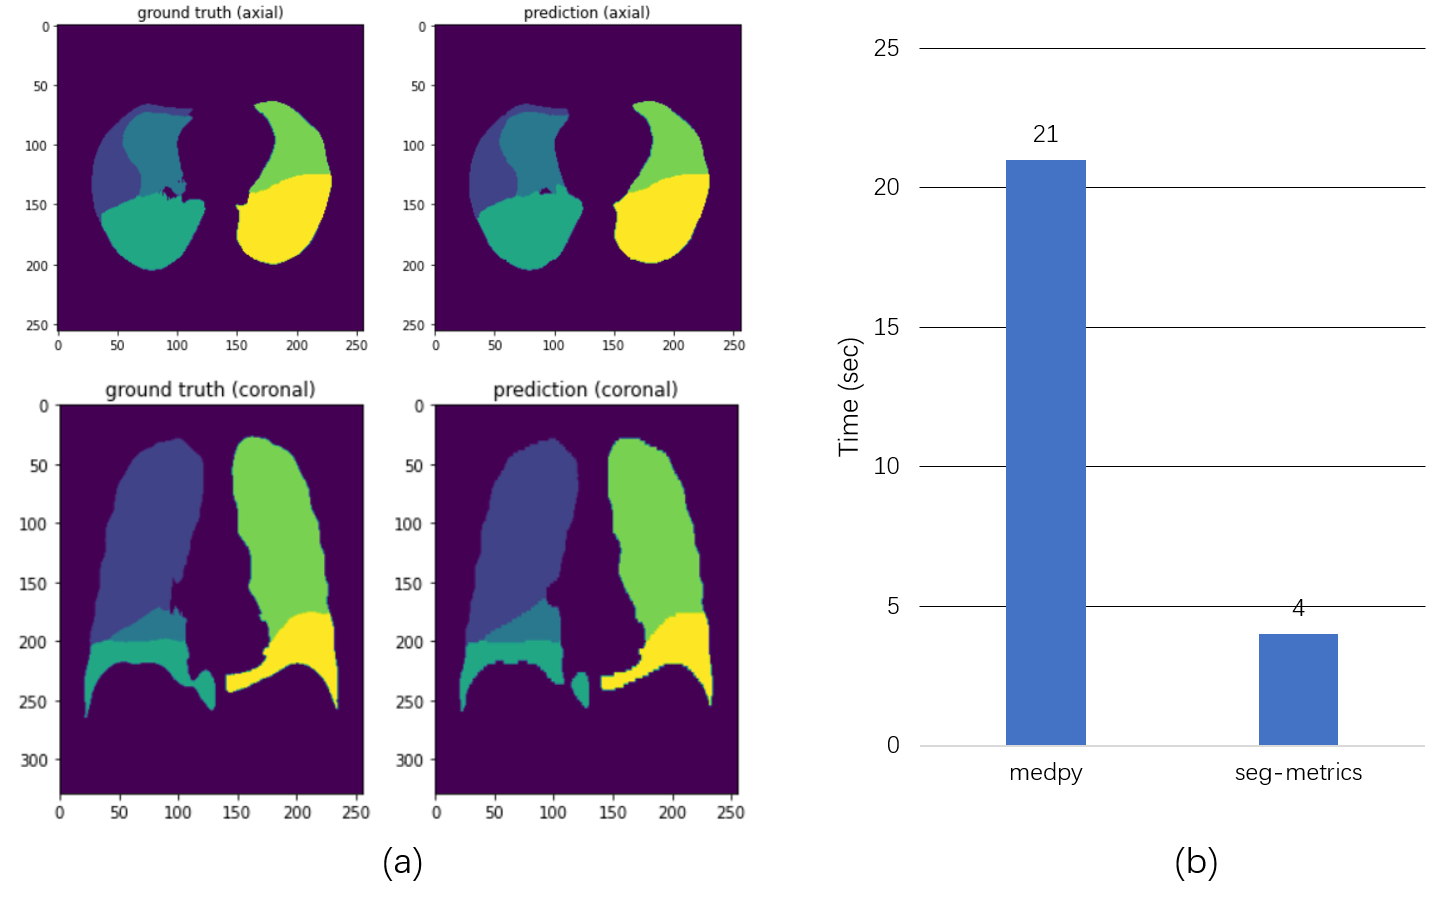
\includegraphics[width=0.75\linewidth]{chapter6//figures/comp.png}
        \caption{Performance comparison between \texttt{medpy} and \texttt{seg-metrics}. (a) Evaluated samples, a 3D lung lobe segmentation results (size: $256 \times 256 \times 256$). Left: ground truth (manually annotated lobes), right: prediction (automatically predicted lobes). (b) Time comparison for the calculation of 'hd', 'hd95' and 'msd'.}
        \label{fig:comp}
    \end{figure}
    
    \item \textbf{More convenient.} \texttt{seg-metrics} can calculate all different metrics in once in one function (shwon below)
    
    \begin{minted}
[frame=single]
{python}
gdth, pred = ...... # load two images
metrics = sg.write_metrics(labels=[1],
                  gdth_img=gdth,
                  pred_img=pred,
                  spacing=spacing,
                  metrics=['hd', 'hd95', 'msd']) # 3 outputs
\end{minted}
    
    while \texttt{medpy} needs to call different functions multiple times which cost more code and time, because the calculation of each 'hd', 'hd95', and 'msd' will always recalculate the distance map which cost much time.
    
\begin{minted}
[frame=single]
{python}
hd = medpy.metric.binary.hd(result=pred, reference=gdth)
hd95 = medpy.metric.binary.hd95(result=pred, reference=gdth)
msd = medpy.metric.binary.asd(result=pred, reference=gdth)
\end{minted}


    \item \textbf{More Powerful.} \texttt{seg-metrics} can calculate multi-label segmentation metrics and save results to .csv file in good manner, but \texttt{medpy} only provides \textbf{binary} segmentation metrics. For instance, if there are 5 labels for an image, our \texttt{seg-metrics} can calculate 5-label metrics by one-line command while \texttt{medpy} needs to at first convert 5-label image to five binary images, then calculate binary metrics one by one, 
\end{itemize}

\section{Limitation and future work}
Because of time limitation, there are still some space for the package to improve. 
\begin{itemize}
    \item Package name. The package name is "seg-metrics" currently, as the abbreviation of "segmentation metrics". But the dash sign "-" in the name introduced some confusion during the installing and usage of the package. Duing the installation, \texttt{pip install seg-metrics} is used. However, users need to used it by \texttt{import seg\_metrics}. The slight difference sometimes make new users confused and easy to make mistakes. This issue is because Python packaging system will automatically convert "\_" to "-" during the installing \cite{dash_underscore_email, dash_underscore_google, dash_underscore_overflow}). Because "segmetrics" has been used by other products, we may consider to change the package name to "metricseg", "metricsrater", "imagesegmetrics", etc. to avoid such issue in the future.
    
    \item Supported file type. Currently, the package supports most medical image formats with suffix of \texttt{.mhd, .mha, .nii, .nii.gz, .nrrd}, etc. Because we receive some users' requests, we will support more image formats (e.g. \texttt{.png, .jpg}) in the future.

    \item Usage guide. Currently, we just list the usage of different metrics, but we did not explain when to use which metrics. In the future, we hope to release a tutorial to users with some examples to show in which case, which metrics are preferable.
    
\end{itemize}


\section{Availability and requirements}
\begin{itemize}
    \item \textbf{Project name:} Seg-metrics
    \item \textbf{Project home page:} \url{https://github.com/Jingnan-Jia/segmentation_metrics}
    \item \textbf{Operating system(s):} Platform independent
    \item \textbf{Programming language:} Python
    \item \textbf{License:} MIT license
    \item \textbf{Any restrictions to use by non-academics:} none
\end{itemize}

\section*{Acknowledgments}
This author was supported by the China Scholarship Council No.202007720110 during the development of this package.
